\chapter{Peierls-Hubbard model}

In cuprate superconductors there are broken symmetries leading to inhomogeneous lattice and electronic structure in the \textit{pseudogap} region of the phase diagram. In this phase the lattice shows a dynamical structure inhomogeneity which can be interpreted in terms of \textit{bipolaronic excitations}. This excitatoins can not be described with the methods based on the Born-Openheimer approximation. The model described here is a representation of the motion of charges (holes) in a O-Cu-O cluster coupled with the ionic motion. It provides a very simple framework to explore the charge dynamics influenced by the lattice vibrations.

In particuar, we have used this model to describe the O(4)-Cu(1)-O(4) cluster for YBCO superconductors.


\section{Description}

The hamiltonian consists of three parts\cite{Salkola1994}:

\begin{equation}\label{full-hamiltonian}H = H_{el} + H_{ph} + H_{el-ph}\end{equation}

The first one is the electronic contribution, the second is due to the phonon energies and the last one is related to the electron-phonon coupling. Explicitly the electronic part is given as

\begin{equation}\label{electronic-part}H_{el} = \sum_n \epsilon_n \rho_n + t\sum_{\langle nn'\rangle\sigma}(c_{n\sigma}^\dagger c_{n'\sigma} + H.c.) + U\sum_n \rho_{n\downarrow}\rho_{n\uparrow}\end{equation}

where $n=1,2,3$ labels each atomic site, $\sigma=\uparrow,\downarrow$ is the spin degree of freedom, $\rho_n$ gives the number of electrons in site $n$. The parameter $t$ represents the "hopping" energy between two adjacent cites $\langle n n'\rangle$ and $c^\dagger_{n\sigma}$, $c_{n\sigma}$ are the creation and anhilation operators for an electron with spin $\sigma$ at site $n$.

The phonon contributions are taken into account as

\begin{equation}\label{phononic-part}H_{ph} = \hbar \omega_{ir}a_{ir}^\dagger a_{ir} + \hbar \omega_R a_R^\dagger a_R\end{equation}

where the subscripts \textit{ir} and \textit{R} refer to the "infrared" (asymmetric) and "Raman" (symmetric) vibrational modes. The operators $a^\dagger$ and $a$ represent the creation and anhilation of a phonon from a given kind.

The electron-phonon interaction part is

\begin{equation}\label{electron-lattice-coupling-part}H_{el-ph} = \lambda_{ir}(a_{ir} + a_{ir}^\dagger)(\rho_3 - \rho_1) + \lambda_R (a_R + a_R^\dagger)(\rho_1 + \rho_3-s_0)\end{equation}

Here the $\lambda$ constants give the strength of the coupling and $s_0$ is a shift to avoid artiificial shinking of the cluster. This contribution is slightly different than the form proposed by Mustre de Leon \textit{et al.}\cite{MustredeLeon1992}, however both can be related by noticing that $3 (\rho_1+\rho_3-4/3)=\rho_1-2\rho_2+\rho_3$.

\subsection{Basis set}

We use the following labelling:

\begin{equation}\label{eq:basis-set}\begin{array}{cccc}  
1= & \uparrow \downarrow & - & - \\
2= & \uparrow & \downarrow & - \\
3= & \uparrow & - & \downarrow \\
4= & \downarrow & \uparrow & - \\
5= & - & \uparrow \downarrow & - \\
6= & - & \uparrow & \downarrow \\
7= & \downarrow & - & \uparrow \\
8= & - & \downarrow & \uparrow \\
9= & - & - & \uparrow \downarrow \end{array}\end{equation}

\section{Nuclei motion}

To model the effect of changing the mass of one atom we model the motion of the nuclei as three masses attached by springs and find the normal modes using classical mechanics A classical model for the motion of the nuclei in the O-Cu-O cluster

\begin{figure}[ht!]
\centering
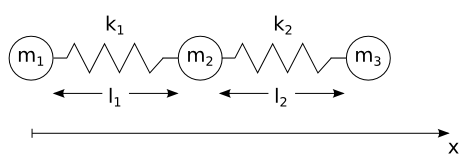
\includegraphics[width=0.8\textwidth]{images/3-masses-2-springs-linear.png}
\caption{Diagram for 3 masses attached with springs representing the nuclei motion.}
\label{fig:3-mases-2-springs}
\end{figure}

Considering the specific case for a O-Cu-O cluster, $m_1=m_3=m_O$, $m_2=m_{Cu}$ and $k_1=k_2\equiv k$, this model gives a symmetric and an antisymmetric frequencies (which we call \textit{Raman} and \textit{infrared} respectively) that depend on the masses: 

\begin{equation}\label{omegaR}\omega_{R}= \sqrt{k/m_O}\end{equation}
\begin{equation}\label{omegair}\omega_{ir} = \sqrt{k(m_{Cu}+2m_O)/m_Om_{Cu}}\end{equation}

Also, the coupling parameters depend on $m_O$<sup>(Reference needed)</sup>:

\begin{equation}\label{ir-coupl-isot}\lambda_{ir}\propto (m_O\omega_{ir})^{-1/2}\end{equation}
\begin{equation}\label{Ram-coupl-isot}\lambda_R\propto (m_O\omega_{R})^{-1/2}\end{equation}

\section{Electronic part}

The electronic part $H_{el}$ is a 9x9 matrix

\begin{equation} \left( \begin{array}{ccccccccc} 
U+2\epsilon &\;\;t\;\;&\;\;0\;\;&\;\;t\;\;&0&\;\;0\;\;&\;\;0\;\;&\;\;0\;\;&0 \\
t&0&t&0&t&0&0&0&0 \\
0&t&2\epsilon &0&0&t&0&0&0 \\
t&0&0&0&t&0&t&0&0 \\
0&t&0&t&U-2\epsilon &t&0&t&0 \\
0&0&t&0&t&0&0&0&t \\
0&0&0&t&0&0&2\epsilon &t&0 \\
0&0&0&0&t&0&t&0&t \\
0&0&0&0&0&t&0&t&U+2\epsilon  \end{array} \right)\end{equation}

that can be diagonalized The electronic excitations projected into the electron-occupation basis.

\section{Isotope effects}

It can be seen from (\ref{omegaR},\ref{omegair},\ref{ir-coupl-isot},\ref{Ram-coupl-isot}) that a change, for example, $^{16}$O $\rightarrow$ $^{18}$O ammounts to a change in the frequencies  $\omega_{ir}$, $\omega_R$ and the couplings $\lambda_{ir}$ and $\lambda_R$. Taking the actual values for copper and oxygen, $m_{Cu}=63.546u$, $m_{^{16}O}=15.995u$ and $m_{^{18}O}=17.999u$ Isotopic change in the O-Cu-O cluster quantum model we obtain:

\begin{equation}\label{omega-ir-isot} \omega^{(16)}_{IR} / \omega^{(18)}_{IR} \simeq 1.039 \end{equation}
\begin{equation}\label{lambda-ir-isot} \lambda_R^{(16)} / \lambda_R^{(18)} \simeq 1.041 \end{equation}

\subsection{Isotopic shift for the excited states}

We define the relative isotopic shift for an excited state $i$ as 

\begin{equation}\label{isot-shift-def-exc}
\Delta_i = \frac{E_i(^{16}O)- E_i(^{18}O)}{E_i(^{16}O)} \times 100 \end{equation}

where the energies $E_i$ are referred to the corresponding ground state.

\subsection{Isotopic shift for the ground state}

For the ground state we define the energy isotopic shift $\Delta_g$ in a similar way but with the energies measured relative to the uncoupled system Isotopic shift of polaron formation energy (that is, the system with $\lambda_{ir}=\lambda_R=0$).

\begin{equation}\label{isot-shift-def-grd}
\Delta_g = \frac{\Delta E_g(^{16}O)- \Delta E_g(^{18}O)}{\Delta E_g(^{16}O)} \times 100 \end{equation}

where $\Delta E_g \equiv E_g - E_g(\lambda_{ir}=0, \lambda_R=0)$. To calculate this energies we need to take into account the \textit{zero-point energy} in (\ref{phononic-part}) which should have been written as 

\begin{equation}\label{phononic-part-complete}
H_{ph} = \hbar \omega_{ir} \left( a_{ir}^\dagger a_{ir} + \frac{1}{2}\right) + \hbar \omega_R\left( a_R^\dagger a_R + \frac{1}{2} \right)\end{equation}


\section{Projection into phonon coordinates}

We can define real coordinates for the two phonon modes in the following way\cite{MustredeLeon1992}

\begin{equation}\label{uR} u_R = \left(\frac{\hbar}{2 m_O \omega_R}\right)^{1/2}(b_R^\dagger + b_R) = \frac{x_3 - x_1}{\sqrt{2}} \end{equation}

\begin{equation}\label{uir} u_{ir} = \left(\frac{\hbar}{2 m_O \omega_{ir}}\right)^{1/2}(b^\dagger_{ir}+b_{ir}) = \frac{ x_1 + x_3 - ( 2 m_O/m_{Cu})x_2}{(2 + 4 m_O/m_{Cu})^{1/2}} \end{equation}

Here $b$ ($b^\dagger$) stands for the annihilation (creation) operator of a phonon mode and $x_i$ is the position of the $i$-th atom in the cluster. It is interesting to look at the wavefunction as a function of $u_R$ and $u_{ir}$.To do this we assume that each phonon mode behaves as if it were a quantum harmonic oscillator, this means that, for each phonon mode, we have energy eigenfunctions of the form

\begin{equation}\label{harmOscProj} \langle u | n \rangle \equiv \psi_n(u) = \frac{1}{\sqrt{2^n n!}} \left(\frac{m \omega}{\pi \hbar}\right)^{1/4}\exp\left(-\frac{m \omega u^2}{2 \hbar}\right) H_n\left( \sqrt{\frac{m \omega}{\hbar}} u \right) \end{equation}

where $H_n$ are the Hermite polynomials. For an arbitrary wavefunction $ | \psi \rangle = \sum_n C_n |n \rangle$ we get $ \langle u | \psi \rangle = \sum_n C_n \langle u | n \rangle$ with $\langle u | n \rangle$ as given above. In our case we have as basis the set ${| e_1, e_2, ir, R \rangle}$ with $e_i$ the position of the $i$-th electron and $ir$, $R$ the number of infrared and Raman phonons respectively. Now, the probability amplitude of findind a state $|\psi\rangle$ proyected into phonon coordinates $(u_{ir},u_R)$ irrespective of the electronic configuration is given by the sum over electronic degrees of freedom The wavefunction in terms of infrared and Raman coordinates:

\begin{equation}\label{phonon-coord-projection} |\psi(u_{ir}, u_R)|^2 = \sum_{e_1}\sum_{e_2} \left(\sum_{n_{ir}} \sum_{n_R} C(e_1, e_2, ir, R) \sqrt{\frac{ m_{ir}^2 m_R^2 \omega_{ir}^2 \omega_R^2 }{2^{(n_{ir} + n_R)}\ n_{ir}!\ n_R!\ \pi \hbar}} \exp \left( - \frac{ \tilde{u}_{ir}^2 + \tilde{u}_R^2 }{2}\right) H_{n_{ir}} ( \tilde{u}_{ir}) H_{n_R}( \tilde{u}_R) \right)^2
\end{equation}

where we have defined 

\begin{equation}\label{uTildeDef}\tilde{u}_x \equiv \sqrt{\frac{m_x\omega_x}{\hbar}}\ u_x\end{equation}

for both phonon modes. In particular, the O-Cu-O cluster the two normal modes' frequencies are given by (\ref{omegaR},\ref{omegair}). With this we identify the reduced masses:

\begin{equation}\label{redMassR} m_R = m_O \simeq 16.0\ u \simeq 2.6568 \times 10^{-26} kg\end{equation}
\begin{equation}\label{redMassIr}m_{ir}=\frac{m_Om_{Cu}}{m_{Cu}+2m_O} \simeq 10.64\ u \simeq 1.7668 \times 10^{-26}kg\end{equation}

And we can estimate the wavefunction in terms of infrared and Raman coordinates.

\begin{equation}\label{uRvstildeuR} u_R = 0.06492\ \tilde{u}_R\ \AA\end{equation}
\begin{equation}\label{uirvstildeuir} u_{ir} = 0.071929\ \tilde{u}_{ir}\ \AA\end{equation}

\subsection{Estimating the split O-Cu distance}

Define $x_1,x_2,x_3$ as usual: the O, Cu and O atomic positons respectively, then the difference $d$ in O-Cu bond lengths is

\begin{equation}\label{bondDiff} d= \left| (x_3 - x_2) - (x_2 - x_1) \right| = \left| x_1 + x_3 - 2x_2 \right| \end{equation}

The $x_i$ coordinates are varying at all times but taking an instant in which $x_2=0$ (can I do that?) and assuming, for example $|x_3|>|x_1|$, we can simplify it to

\begin{equation}\label{bondDiffSimpl}d=x_1+x_3\end{equation}

And, from $u_{ir}$'s definition in (\ref{uir}),

\begin{equation}\label{uirSimpl} u_{ir}=\frac{x_1+x_3}{\left( 2+4 m_O/m_{Cu} \right)^{1/2}}\end{equation}

Now we substitute (\ref{bondDiffSimpl}) into (\ref{uirSimpl}) to obtain

\begin{equation}\label{uirvsd}u_{ir}=\frac{d}{\left( 2+4 m_O/m_{Cu} \right)^{1/2}} \end{equation}

or, solving for $d$,

\begin{equation}\label{dvsuir}d=\sqrt{2}\left(1 + 2\frac{m_O}{m_{Cu}} \right)^{1/2}u_{ir}\end{equation}

\section{Projection into states with definite electron occupation numbers}

We obtain states with definite electron occupation numbers by summing over phononic degrees of freedom. This states are labelled by (\ref{eq:basis-set}).
